% !TEX root = ../thesis.tex
\section{Aplikace obecného systému rozpoznávání a dosažené výsledky}
\label{chap:construction:results}

Z provedené analýzy plyne, že získaný EL korpus je odlišný od \uv{standardního} řečového korpusu, který se běžně používá k trénování obecných akustických modelů.
Tyto modely jsou nezávislé na řečníkovi a vyznačují se robustností.
Je tedy otázka, zda bude obecný akustický model schopen pracovat s EL daty.

Za účelem ověření hypotézy byl vytvořen TDNN akustický model (popsaný v části \ref{chap:asr:acoustic:DNN}), který byl natrénován daty z korpusu čítajícího $1000$ hodin promluv od velkého počtu řečníků.
Celkový počet HMM stavů je \textbf{XXXX}.

Jazykový model je založen na trigramech slov a k jeho natrénování posloužil textový korpus čítající velké množství novinových článků, webových reportáží, filmových titulků a dalších textových záznamů.
Slovník jazykového modelu čítá více než $1$ milion unikátních slov.

Testovacím vstupem vytvořeného ASR systému jsou data z EL korpusu.
Celková slovní přesnost, počítaná podle vzorce (\ref{eq:asr:decoding:acc}), dosáhla hodnoty $18,49\ \%$\footnote{Dosaženo na state-of-the-art ASR systému v době psaní práce. V době vytvoření EL korpusu (kolem roku 2011) převládaly HMM-GMM akustické modely. Tento systém dosáhl přesnosti na slovech $12,59\ \%$.}.
Dosažený výsledek zřetelně ilustruje odlišnost EL domény, protože obecný na řečníkovi nezávislý systém s rozsáhlým jazykovým modelem není schopen obstojně rozpoznat EL promluvu.

Pokud jsou k natrénování akustického modelu (taktéž využívajícího TDNN síť) použita pouze data\footnote{Korpus byl náhodně rozdělen na trénovací a testovací sadu v poměru $90\ \%\ (10h41m44s)$ trénovací a $10\ \%\ (1h00m58s)$ testovací sada. Toto rozděleni je použito ve všech experimentech.} z EL korpusu, tak výsledná slovní přesnost dosáhla hodnoty $83,33\ \%$, opět počítáno podle vzorce (\ref{eq:asr:decoding:acc}).
Jazykový model je identický jako v případě obecného systému.
Dosažený výsledek demonstruje výhodu vytvoření individuálního modelu z EL nahrávek.
Zároveň ukazuje schopnost akustického modelu přizpůsobit se specifikům EL řeči.
Přestože je výstup individuálního modelu výrazně přesnější než obecného modelu zpracovávající EL promluvy, tak zdaleka nedosahuje výsledků srovnatelných s nejlepšími ASR systémy, které jsou schopny v ideálních podmínkách dosahovat více než $90\ \%$ slovní přesnosti.


%Z dosaženého výsledku je patrné, že EL doména je diametrálně odlišná od běžné řeči, pro které jsou ASR systémy vytvářeny. Navíc, pokud se vezme v potaz náročnost získání potřebných dat pro natrénování obecného modelu, tak se jako jediná schůdná varianta jeví vytváření individuálních modelů pro každého řečníka. To znamená, že model je trénovaný pouze z dat odpovídající konkrétnímu řečníkovi a často i účelu použití. K vytvoření takového modelu je zapotřebí řádově méně dat, při dosažení podobného výkonu. Stinnou stránkou je případná menší robustnost modelu. Čistě logicky tento model bude fungovat pouze s konkrétním řečníkem a ještě jen v situacích, které odpovídají trénovacím datům. U řečníků s EL může navíc hrát velký vliv samotný EL. Již při nahrávání se ukázalo, že jeho pozice může nepříznivě ovlivnit kvalitu řeči. Tento problém by však neměl významně ovlivňovat kvalitu modelu, protože tento fenomém je obsažen v datech.

\subsection{Hledání optimálních parametrů baseline modelu}
\label{chap:construction:results:baseline}

%Co se však ukázalo jako potencionálně problematické, je stabilita parametrů produkované řeči v dlouhodobém časovém úseku. Více o tomto problému pak v části \ref{chap:construction:normalization:quality}. K zodpovězení nejdůležitější otázky, jestli takový model vůbec může fungovat, stačí získaná data z první etapy nahrávání a ta obsahují řeč s relativně konzistentními parametry.

V rámci ověřování funkčnosti individuálního modelu je vhodné otestovat různé kombinace parametrů modelu za účelem nalezení optimálních hodnot.
Hlavními uvažovanými hyperparametry jsou vzorkovací frekvence audio nahrávek a počet HMM stavů.
Pořízené nahrávky mají vzorkovací frekvenci rovnu $44,1\ kHz$.
Pro úlohu rozpoznávání EL řeči je to však zbytečně vysoká frekvence, protože nejhodnotnější informace je u EL řeči obsažena ve frekvenčním pásmu do $4\ kHz$.
Vyšší frekvence ovlivňuje především zabarvení hlasu a další individuální charakteristiky \cite{Psutka2006}.
Samotná EL řeč má svá specifika, proto se otevírá otázka volby vhodné vzorkovací frekvence.
% však obsahuje věci, které běžná řeč neobsahuje a tak je otázka, zde vhodnější vzorkovací frekvence rovna $8\ kHz$ nebo lépe $16\ kHz$.

Jak bylo řečeno výše, počet stavů modelu ovlivňuje množství modelovaných trifónů.
Čím více akustických jednotek je modelováno, tím více musí mít HMM model unikátních stavů.
Od počtu unikátních stavů se odvíjí rozsah množiny trénovacích dat potřebný pro  natrénování robustního modelu.
Pro účely výběru optimální struktury modelu bylo uvažováno $1024,\ 2048$ a $4096$ stavů.
%Jen pro vysvětlení je dobré zmínit, že HMM stav představuje model jedné uvažované akustické jednotky (nebo skupiny jednotek s podobnými parametry). Počet stavů nám tedy říká, kolik takových jednotek model dokáže rozlišit. Čím více stavů, tím více jednotek (menších skupin) je modelováno. Teoreticky tak model s více stavy je lepší. Nicméně k natrénování jednotky je potřeba určité množství dat, a tím pádem je pro model s vyšším počtem stavů logicky potřeba větší množství trénovacích dat. Samozřejmě fonetická sada neobsahuje $4096$ fonémů, neobsahuje ani $1024$ fonémů\footnote{Ve skutečnosti obsahuje 42 českých fonémů.}. U těchto modelů se pak používá nějaký druh \textit{n-gramové} reprezentace fonémů, nejčastěji pak trifóny.
Jestliže byly uvažovány dvě hodnoty vzorkovací frekvence $8\ kHz$ a $16\ kHz$, bylo natrénováno $6$ modelů.
K vytvoření akustických modelů byl použit nástroj HTK-Toolkitu ve verzi v3.4., který je určen k vytváření HMM modelů.
Při trénování byl nejprve vytvořen monofónový akustický model s jedním Gaussiánem pro každý stav.
Ten slouží jako základ pro trifónové modely.
Výsledný trifónový model využívá směs Gaussiánů v souladu s částí \ref{chap:asr:acoustic:GMM}.
Celý proces trénování je znázorněn na obr. \ref{fig:construction:results:baseline:hmm:training}.

\begin{figure}[hbpt]
  \centering
  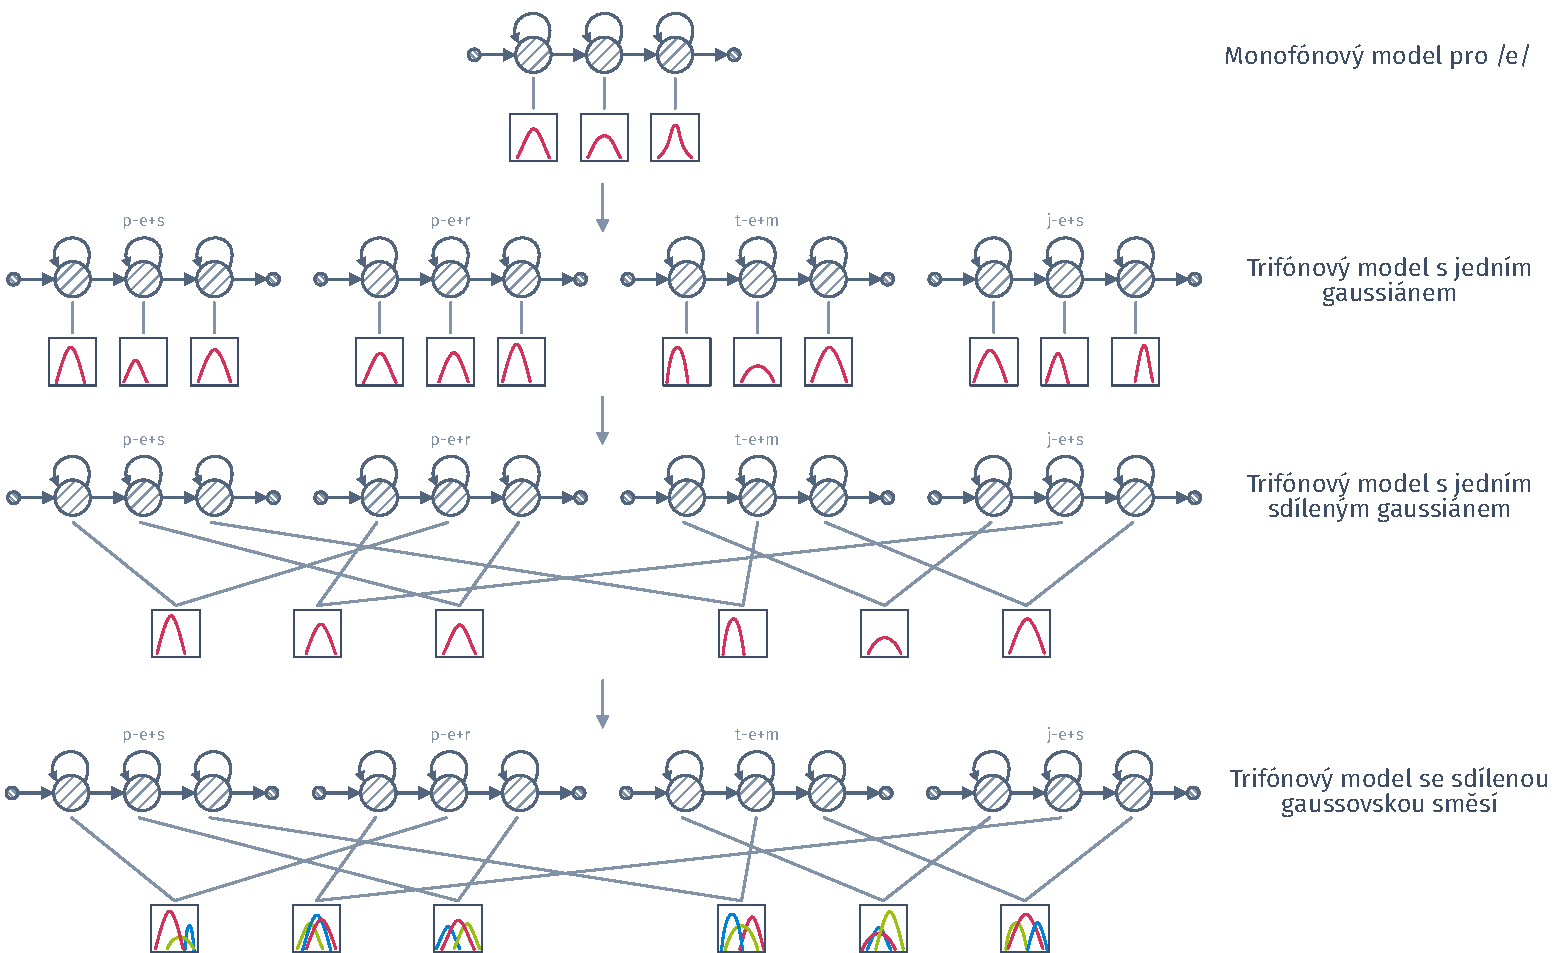
\includegraphics[width=0.9\textwidth]{./ch5-construction/img/hmm-training.pdf}
  \caption{Princip trénování HMM-GMM modelu.}
  \label{fig:construction:results:baseline:hmm:training}
\end{figure}

Cílem popsané procedury je nalezení vhodných parametrů baseline modelu, zejména pak toho akustického.
K tomu je potřeba minimalizovat vliv jazykového modelu.
Z tohoto důvodu je použit speciální zerogramový jazykový model.
Standarně se předpokládá, že základní jednotkou jazykového modelu je slovo.
Pro ně jsou počítány četnosti z trénovacích dat a vytvořen model.
Obecně ale není nutné, aby základní jednotkou bylo slovo. V případě experimentů s EL řečí je mnohem výhodnější vytvořit model, jehož základní jednotkou je foném, protože právě foném je výstupem akustického modelu.
Výstupem ASR systému tak bude sekvence fonémů, která z praktického pohledu není úplně užitečná, ale pro testování vlastností akustického modelu se hodí dokonale.
V rámci této práce je takovýto model označován jako fonémový zerogramový jazykový model.
Velikost slovníku tohoto modelu odpovídá velikosti fonémové sady, a tedy lze pravděpodobnost výskytu libovolného fonému stanovit jako $P(w_n) = 1/N$\footnote{Označení $w_n$ může evokovat použití slov u jazykového modelu. Změna písmena by však mohla vést ke zmatení čtenáře, protože by byla použita nestandardní notace. Z tohoto důvodu je i pro speciální model použito označení fonémů $w_n$.}, kde $N=40$.
Výsledná přesnost je tedy závislá pouze na akustickém modelu.
Akustická data byla parametrizována pomocí MFCC s 26 filtry, 12 kepstrálními koeficienty a energií.
Příznakový vektor obsahuje první i druhou derivaci těchto koeficientů.
Podrobněji je parametrizace založená na procesu slyšení popsána v části \ref{chap:asr:parametrization:hearing}.


% Funkce ASR systému lze popsat rovnící

% \begin{equation}
%   \argmax_W p\left(W | O\right) = \argmax_W p\left(O | W\right) p\left(W\right),
% \end{equation}

%\noindent kde $\boldsymbol{O}$ reprezentuje sekvenci akustických příznaků a $W$ výstupní sekvenci znaků\footnote{Znakem tu může být myšleno písmeno, případně slovo.}. $P\left(O | W\right)$ je pravděpodobnost generování korektní pozorované sekvence, tedy korektní k akustickému modelu ASR systému. Pravděpodobnost $P\left(W\right)$ je apriorní pravděpodobnost konkrétní sekvence znaků $W$, jinými slovy jazykový model. K získání výsledků je tedy potřeba mít i tento model.

%Ten však není níjak ovlivněn řečníkem (pouze doménou použití systému) a není jej třeba upravovat pro potřeby řečníka s EL. Cílem experimentu je ověření funkčnosti ASR a nalezení optimálních parametrů akustického modelu. Z tohoto důvodu je potřeba co nejvíce eliminovat vliv jazykového modelu na celkovém výkonu ASR systému. Jak bylo zmíněno, funkcí $p\left(W\right)$ je určení nejpravděpodobnější sekvence znaků. Pravděpodobnostní rozložení je získáno z velkého množství trénovacích textů. Toto natrénované rozložení by však velmi ovlivnilo výsledky experimentů, a proto je použít zerogramový monofónový model. Ten se vyznačuje tím, že všechny prvky slovníku mají stejnou pravděpodobnost rovnu $P(w_n) = \frac{1}{N}$, kde $N$ je počet položek ve slovníku. Monofónový model je navíc zvolen z toho důvodu, že fonetická sada je známa a obsahuje malý počet jednotek. Z pohledu jazykového modelu má libovolný výstup z akustického modelu stejnou pravděpodobnost výskytu, a tím pádem se jazykový model nijak nepřispívá k celkové kvalitě ASR systému.

V~tab. \ref{tab:construction:experiment:gmm} jsou uvedeny dosažené výsledky HMM-GMM modelů.
Opět se potvrdilo, že individuální ASR systém s EL daty může fungovat.
Pokud dosažené výsledky porovnáme s výsledky obecného modelu ($Acc_{word} = 18,49\ \%)$, tak i zde je vidět rapidní nárůst přesnosti ($78,63\ \%$ u nejhoršího individuálního GMM modelu).
Ze získaných výsledků je zřejmé, že volba vzorkovací frekvence má významný dopad na přesnost rozpoznávání.
Při použití vyšší vzorkovací frekvence, zde $16\ kHz$, je vhodnější.
Oproti $8\ kHz$ bylo dosaženo zlepšení přesnosti o $1,41\ \%$ absolutně, tedy téměř $7\ \%$ relativně.
Dodatečné experimenty ukázaly, že použití vyšší vzorkovací frekvence než $16\ kHz$ přinese jen zanedbatelné zlepšení.

Dále se ukázalo, že počet stavů nehraje tak zásadní roli při posuzování kvality akustického modelu, jako vzorkovací frekvence.
Z testované množiny počtu stavů dosáhl nejlepšího výsledku model, který měl maximálně $4096$ stavů, nicméně oproti modelu s $1024$ stavy je nárůst přesnosti pouze $0,4\ \%$ absolutně v případě vzorkovací frekvence $16\ kHz$, což není tak významné.
Logicky se nabízí otázka, proč nezkusit ještě více stavů.
Odpověď se skrývá ve skutečném počtu stavů modelu s maximálním počtem $4096$ stavů.
Slovíčko \uv{maximálním} je zde podstatné.
Algoritmus trénování akustického modelu se snaží rozdistribuovat všechny možné akustické jednotky (v tomto případě trifóny) do maximálního počtu stavů.
Pokud chceme dosáhnout menšího počtu stavů než jednotek, dochází k určité formě shlukování (za pomocí fonetického rozhodovacího stromu) \cite{Holmes2001}.
Pokud je k dispozici dostatek dat k natrénování konkrétního shluku, je tento shluk akceptován, pokud jich není dostatečné množství, je tento shluk spojen s jiným, který je svými parametry nejblíže.
V případě, že je k dispozici dostatek dat k natrénování maximálního počtu stavů má model tento počet stavů.
Pokud není dostatek dat, může mít model méně stavů.
U modelu s maximálním počtem $4096$ stavů je skutečný počet stavů $3257$, tzn. i kdyby se trénoval model s $8192$ stavy, tak by se tato hodnota změnila jen velmi málo.

%Pro doplnění, fonémový akustický model dosáhl přesnosti $54,49\ \%$ pro $8\ kHz$ a $62,30\ \%$ pro $16\ kHz$.

\begin{table}[htpb]
  \centering
  \def\arraystretch{1.5}
  \pgfplotstabletypeset[
    col sep=semicolon,
    string type,
    columns/model/.style={column name={Počet HMM stavů}, column type={c}},
    columns/8k/.style={column name={8 kHz}, column type={r}},
    columns/16k/.style={column name={16 kHz}, column type={r}},
    every head row/.style={
      before row={
        \toprule & \multicolumn{2}{c}{$Acc_{p}\ [\%]$} \\
      },
      after row={
        \cmidrule(r){1-1}
        \cmidrule(l){2-3}
      }
    },
    every last row/.style={after row={\bottomrule}},
  ]{./ch5-construction/tabs/01-frequency.csv}
  \caption{Vliv frekvence na kvalitu modelu.}
  \label{tab:construction:experiment:gmm}
\end{table}

Hledání optimálních parametrů baseline modelu bylo realizováno na přelomu let $2013$ a $2014$.
V tuto dobu byly stále dominantní GMM modely.
Z tohoto důvodu byl později tento experiment zopakován s HMM-DNN akustickým modelem.
Vstupem modelu byla stejná MFCC parametrizace s 26 filtry, 12 kepstrálními koeficienty plus energie, delta a delta-delta příznaky.
Tato parametrizace je provedena na mikrosegmentu $t$ a jeho okolí $t-5$ a $t+5$.
Každý mikrosegment má délku $10\ ms$.
Samotná síť se skládá z 6 vrstev, každá s 4096 neurony, výstupní vrstva je typu softmax s dimenzí rovnou počtu HMM stavů.
Dosažené výsledky jsou v tab. \ref{tab:construction:experiment:dnn}.
Z nich je patrné, že nalezené optimální hyperparametry jsou shodné i při použití DNN.
Nicméně je zde i zřejmý důvod následné dominance HMM-DNN modelů.
Fungují totiž výrazně lépe.
Pouhou náhradou GMM za DNN bylo dosaženo zlepšení.
Hodnoty přesnosti baseline modelu jsou tedy pro GMM $Acc_{p}^{GMM} = 81,20\ \%$ a pro DNN $Acc_{p}^{DNN} = 85,23\ \%$. To odpovídá zlepšení o $4\ \%$ absolutně oproti nejlepšímu GMM výsledku, viz tab. \ref{tab:construction:experiment:gmm} a \ref{tab:construction:experiment:dnn}.

%experiment byl realizován na přelomu let $2013$ a $2014$, kdy ještě $ASR$ modelům dominovaly \textit{HMM-GMM} modely, byl později zopakován s \textit{HMM-DNN} modely, které dosahují ještě vyšších přesností.

%Více o \textit{HMM-DNN} v části \ref{chap:construction:normalization:corpus}. Výsledky těchto modelů jsou v tab. \ref{tab:construction:experiment:dnn}, z nich je vidět, že i v této oblasti neuronové sítě jasně dominují.

\begin{table}[htpb]
  \centering
  \def\arraystretch{1.5}
  \pgfplotstabletypeset[
    col sep=semicolon,
    string type,
    columns/model/.style={column name={Počet HMM stavů}, column type={c}},
    columns/8k/.style={column name={8 kHz}, column type={r}},
    columns/16k/.style={column name={16 kHz}, column type={r}},
    every head row/.style={
      before row={
        \toprule & \multicolumn{2}{c}{$Acc_{p}\ [\%]$} \\
      },
      after row={
        \cmidrule(r){1-1}
        \cmidrule(l){2-3}
      }
    },
    every last row/.style={after row={\bottomrule}},
  ]{./ch5-construction/tabs/01-frequency_dnn.csv}
  \caption{Vliv frekvence na kvalitu modelu využívajícího DNN.}
  \label{tab:construction:experiment:dnn}
\end{table}

\subsection{Redukce fonetické sady}
\label{chap:construction:results:reduction}

Při mluvení je elektrolarynx permanentně zapnutý, a to i v případě neznělých fonémů.
Toto má vliv na jejich průběh, podrovněji v části v \ref{chap:construction:analysis}.
Nabízí se tak předpoklad, že všechny neznělé fonémy mají podobu znělých párových fonémů, a tím pádem je možné redukovat fonetickou sadu.
V důsledku redukce fonetické sady by došlo ke snížení perplexity modelu.
Rozhodnutí, zda se jedná o variantu slova obsahující znělý nebo neznělý foném, je pak přenecháno jazykovému modelu.

K ověření tohoto předpokladu je potřeba provést experimentálního ověření.
Myšlenka experimentu je jednoduchá.
Je potřeba natrénovat několik modelů lišících se pouze tím, jaký fonetický pár (viz tab. \ref{tab:construction:reduction:pairs}) je použit pro redukci fonetické sady.
V rámci experimentu jsou uvažovány tyto případy:

\begin{itemize}
  \item \textit{Baseline} - standardní model s plnou fonetickou sadou.
  \item $/f/ \rightarrow /v/$ - foném $/f/$ je nahrazen fonémem $/v/$.
  \item $/k/ \rightarrow /g/$ - foném $/k/$ je nahrazen fonémem $/g/$.
  \item $/s/+/\check{s}/ \rightarrow /z/+/\check{z}/$ - foném $/s/$ $\left(/\check{s}/\right)$ je nahrazen fonémem $/z/$ $\left(/\check{z}/\right)$.
  \item $/t/+/\text{\textit{ť}}/ \rightarrow /d/+/\text{\textit{ď}}/$ - foném $/t/$ $\left(/\text{\textit{ť}}/\right)$ je nahrazen fonémem $/d/$ $\left(/\text{\textit{ď}}/\right)$.
  \item \textit{Náhrada všech} - všechny uvažované neznělé fonémy jsou nahrazeny znělým ekvivalentem.
\end{itemize}

\begin{table}[htpb]
  \centering
  \def\arraystretch{1.5}
  \pgfplotstabletypeset[
    col sep=comma,
    string type,
    columns/unvoiced/.style={column name={Neznělé fonémy}, column type={c}},
    columns/voiced/.style={column name={Znělé fonémy}, column type={c}},
    every head row/.style={
      before row={\toprule},
      after row={\cmidrule(r){1-1}\cmidrule(l){2-2}}
    },
    every last row/.style={after row={\bottomrule}},
  ]{./ch5-construction/tabs/phonemes_pairs.csv}
  \caption{Korespondující páry fonémů.}
  \label{tab:construction:reduction:pairs}
\end{table}

\noindent Pro porovnání jsou stejné modely vytvořeny i pro zdravého řečníka.
U něj by při libovolné redukci fonetické sady mělo dojít ke zhoršení oproti \textit{baseline} modelu.

K natrénování akustických modelů byly použity korpusy čítající 5000 vět\footnote{Pro oba řečníky byly použity stejné věty pocházející z databáze popsané v \cite{Radova2000}.}, což představuje více než 10 hodin řeči pro každého řečníka.
Akustická data byla parametrizována pomocí MFCC s 26 filtry a 12 kepstrálními koeficienty a energií.
Dále vektor parametrů obsahuje delta a delta-delta příznaky.
To dohromady tvoří vektor 39 příznaků pro každých 10 ms nahrávky \cite{Psutka2007}.

V rámci experimentu byly otestovány dva přístupy.
%vzájemně se lišící řečovou jednotkou.
V prvním případě se jednalo o monofónový akustický model, v druhém případě byl testován trifónový.
U obou přístupů je řečová jednotka reprezentována pětistavovým HMM-GMM modelem se spojitou výstupní pravděpodobnostní funkcí pro každý stav.
% , viz \ref{chap:asr:acoustic:HMM}.
Pro určení optimálních parametrů modelu pro EL byly využity poznatky uvedené v  části \ref{chap:construction:results:baseline}. P
ro zdravého řečníka je pro každou část experimentu vytvořeno několik modelů lišících se počtem stavů a Gaussovských směsí.
Všechny akustické modely jsou natrénovány pomocí HTK-Toolkitu v3.4.
Celkem bylo vytvořeno 24 akustických modelů, 12 pro EL řečníka (6 monofónových a 6 trifónových) a 12 pro zdravého řečníka.

Pro otestování modelů byla vytvořena testovací sada čítající 500 vět náhodně vybraných z původních korpusů (pro oba řečníky stejná).
Testovací sada tak představuje přibližně 1 hodinu řeči pro každého řečníka.
V rámci tohoto experimentu jsou uvažovány dva jazykové modely

\begin{enumerate}
  \item \textit{zerogramový jazykový model} - v tomto případě mají všechna slova v modelu stejnou pravděpodobnost výskytu $P_r(w_n|w_1,\dots,w_{n-1}) = \frac{1}{N}$, kde $N$ je počet slov ve slovníku. Konkrétně pro $N = 2885$, odpovídá perplexita modelu hodnotě $2885$. Testovací slovník je vytvořen z testovací sady, model tedy neobsahuje OOV\footnote{Out-of-vocabulary (OOV) - slova, která nejsou obsažena ve slovníku jazykového modelu.}.
  \item \textit{trigramový jazykový model} - u tohoto modelu odpovídá pravděpodobnost výskytu následujícího slova $P_r(w_n|w_1,\dots,w_{n-1})~=~P(w_n|w_{n-2}, w_{n-1})$. K získání $P(w_n|w_{n-2}, w_{n-1})$ posloužil SRILM Toolkit s Kneser-Ney vyhlazováním\footnote{Vyhlazování slouží k vyřešení problému s OOV, kdy trénovací data neobsahovala tato OOV, a proto není k dispozici $p(w_n|w_{n-2}, w_{n-1})$.} \cite{Stolcke2002}, které se podle \cite{Prazak2008} ukázalo jako optimální pro tyto typy modelů. Jako trénovací data byly použity texty z novinových článků, webových stránek a přepisů televizních pořadů. Celkem model obsahuje 360 tisíc nejvíce frekventovaných slov. OOV bylo $3,8 \%$ a perplexita $3380$.
\end{enumerate}

\noindent V kombinaci s vytvořenými akustickými modely to představuje 4 dílčí experimenty.
Jen pro doplnění je nutné poznamenat, že přesnost modelů je vyhodnocována na slovech.
%, oproti fonémovému baseline modelu v \ref{chap:construction:results:baseline}.

V tab. \ref{tab:construction:reduction:01} a \ref{tab:construction:reduction:02} jsou shrnuty dosažené výsledky pro monofónový akustický model a zerogramový jazykový model, resp. trigramový jazykový model.
V obou případech se potvrdilo očekávané chování přesnosti modelu u zdravého řečníka.
Redukcí fonetické sady je omezena komplexita modelu, a tím pádem dochází ke zhoršení přesnosti.
Překvapivé mohou být horší výsledky u zdravého řečníka uvedené v tab. \ref{tab:construction:reduction:02}.
Toto chování může být vysvětleno vyšší perplexitou trigramového jazykového modelu v kombinaci s relativně jednoduchým monofónovým akustickým modelem.

U EL řečníka je vidět dílčí zlepšení u 2 modelů (tab. \ref{tab:construction:reduction:01}), resp. 1 modelu v případě trigramového modelu (tab. \ref{tab:construction:reduction:02}).
Ve většině případů však redukce fonetické sady vedla ke zhoršení přesnosti.
Při použití trigramového jazykového modelu došlo obecně ke zlepšení výkonu systému i přesto, že tento model má vyšší perplexitu.
To nasvědčuje tomu, že pro tuto úlohu je monofónový akustický model příliš jednoduchý.

\begin{table}[htpb]
  \centering
  \def\arraystretch{1.5}
  \pgfplotstabletypeset[
    col sep=semicolon,
    string type,
    columns/model/.style={column name=Model, column type={c}},
    columns/normal/.style={column name={Zdravý}, column type={r}},
    columns/el/.style={column name={EL}, column type={r}},
    every head row/.style={
      before row={
        \toprule & \multicolumn{2}{c}{$Acc_{w}\ [\%]$} \\
      },
      after row={
        \cmidrule(r){1-1}
        \cmidrule(l){2-3}
      }
    },
    every last row/.style={after row={\bottomrule}},
  ]{./ch5-construction/tabs/reduction_01.csv}
  \caption[Vliv redukce na přesnost ASR s mono. AM. a zerogram LM.]{Vliv redukce fonetické sady na přesnost ASR systému s monofoním akustickým a zerogramovým jazykovým modelem ($N=2885$) pro zdravého a EL řečníka.}
  \label{tab:construction:reduction:01}
\end{table}

\begin{table}[htpb]
  \centering
  \def\arraystretch{1.5}
  \pgfplotstabletypeset[
    col sep=semicolon,
    string type,
    columns/model/.style={column name=Model, column type={c}},
    columns/normal/.style={column name={Zdravý}, column type={r}},
    columns/el/.style={column name={EL}, column type={r}},
    every head row/.style={
      before row={
        \toprule & \multicolumn{2}{c}{$Acc_{w}\ [\%]$} \\
      },
      after row={
        \cmidrule(r){1-1}
        \cmidrule(l){2-3}
      }
    },
    every last row/.style={after row={\bottomrule}},
  ]{./ch5-construction/tabs/reduction_02.csv}
  \caption[Vliv redukce na přesnost ASR s mono. AM. a 3-gram LM (N=360k).]{Vliv redukce fonetické sady na přesnost ASR systému s monofonním akustickým a trigramovým jazykovým modelem obsahujícím 360 tisíc slov pro zdravého a EL řečníka.}
  \label{tab:construction:reduction:02}
\end{table}


V tab. \ref{tab:construction:reduction:03} a \ref{tab:construction:reduction:04} jsou pak uvedeny výsledky pro trifónový akustický model se zerogramovým resp. trigramovým jazykovým modelem.
Stejně jako u předchozích dvou experimentů, tak i zde, je vidět, že redukce fonetické sady vede u zdravého řečníka vždy ke zhoršení přesnosti modelu.
Z uvedených výsledků je patrné, že trifónový akustický model dosahuje výrazně lepších výsledků než monofonní model.
Lze se domnívat, že zhoršení kvality rozpoznávání u EL řečníka v tab. \ref{tab:construction:reduction:03} je s nejvyšší pravděpodobností způsobeno využitím fonetických stromů v AM, protože v trénovací sadě není dostatek dat pro všechny možné varianty trifónů.
Tím pádem model pro určité trifóny vrací špatné sekvence znaků.
Zerogramový jazykový model pak nedokáže pomoci, protože všechna slova mají stejnou pravděpodobnost výskytu $P_r(w_n|w_1,\dots,w_{n-1}) = \frac{1}{2885}$.
Tím pádem dochází k rozpoznání špatného slova, tedy ke snížení celkové přesnosti rozpoznávání.
Tuto domněnku potvrzuje rapidní zlepšení v případě trigramového jazykového modelu (tab. \ref{tab:construction:reduction:04}), kde již jazykový model významně přispívá k přesnosti modelu.

\begin{table}[htpb]
  \centering
  \def\arraystretch{1.5}
  \pgfplotstabletypeset[
    col sep=semicolon,
    string type,
    columns/model/.style={column name=Model, column type={c}},
    columns/normal/.style={column name={Zdravý}, column type={r}},
    columns/el/.style={column name={EL}, column type={r}},
    every head row/.style={
      before row={
        \toprule & \multicolumn{2}{c}{$Acc_{w}\ [\%]$} \\
      },
      after row={
        \cmidrule(r){1-1}
        \cmidrule(l){2-3}
      }
    },
    every last row/.style={after row={\bottomrule}},
  ]{./ch5-construction/tabs/reduction_03.csv}
  \caption[Vliv redukce na přesnost ASR s trif. AM. a zerogram. LM.]{Vliv redukce fonetické sady na přesnost ASR systému s trifónovým akustickým a zerogramovým jazykovým modelem pro zdravého a EL řečníka.}
  \label{tab:construction:reduction:03}
\end{table}

\begin{table}[htpb]
  \centering
  \def\arraystretch{1.5}
  \pgfplotstabletypeset[
    col sep=semicolon,
    string type,
    columns/model/.style={column name=Model, column type={c}},
    columns/normal/.style={column name={Zdravý}, column type={r}},
    columns/el/.style={column name={EL}, column type={r}},
    every head row/.style={
      before row={
        \toprule & \multicolumn{2}{c}{$Acc_{w}\ [\%]$} \\
      },
      after row={
        \cmidrule(r){1-1}
        \cmidrule(l){2-3}
      }
    },
    every last row/.style={after row={\bottomrule}},
  ]{./ch5-construction/tabs/reduction_04.csv}
  \caption[Vliv redukce na přesnost ASR s trif. AM. a 3-gram LM (N=360k).]{Vliv redukce fonetické sady na přesnost ASR systému s trifónovým akustickým a trigramovým jazykovým modelem s 360 tisíc slov pro zdravého a EL řečníka.}
  \label{tab:construction:reduction:04}
\end{table}

U obou experimentů s trifónovým akustickým modelem došlo ke zlepšení u dvou modelů (tab. \ref{tab:construction:reduction:03} a \ref{tab:construction:reduction:04}). Naproti tomu redukce fonetické sady vedla ve většině případů stejně jako v případě monofónového modelu ke zhoršení přesnosti rozpoznávání.


Ze získaných výsledků je možné usoudit, že redukce fonetické sady může vést ke zlepšení přesnosti.
Nicméně předpoklad, že všechny neznělé fonémy jsou shodné se svými znělými ekvivalenty se ukázala jako mylná.
Zároveň také není možné říci, že náhrada např. dvojice $/s/$ a $/\check{s}/$  za každých okolností to povede k lepším výsledkům.
Při hlubší analýze se ukázalo, že velmi záleží na kontextu daného fónemu, ten totiž velmi ovlivňuje jeho podobu.
Řeč představuje spojitou formu signálu a při vyslovování různých slov obsahujících stejný foném s odlišným okolím  může dojít k odchylkám například v artikulaci, příkladem může být dvojice slov \textit{hrad} a \textit{had}.
Toto pozorování ověřil i dodatečný experiment, ve kterém byl u náhrady $/s/$ za $/z/$ vynechán trifón \textit{b-s+t}, který je například ve slově \textit{obstát}.
Díky vynechání tohoto jediného trifónu byla výsledná nejlepší přesnost u trifónového akustického modelu $83,39\ \%$ (původně $83,28\ \%$) v případě zerogramového jazykového modelu a $88,44\ \%$ (původně $88,31\ \%$) v případě trigramového modelu.
Přestože se jedná o marginální zlepšení, tak ho bylo docíleno jedním trifónem.
Bohužel určení toho, jaké trifóny vynechat z nahrazování není v žádném případě triviální úloha.

Zajímavý je také rozdíl mezi přesností modelu pro zdravého řečníka a EL řečníka.
Přestože se v obou případech jedná o individuální modely šité \uv{na míru} řečníkovi, tak průměrný rozdíl v přesnosti rozpoznávání činí $6,24\ \%$ absolutně, resp. $40,38\ \%$ relativně.
To značí, že je potřeba se zabývat myšlenkou úpravy akustického modelu za účelem dosažení lepších výsledků.
V ideálním případě dokonce srovnatelných s modely pro zdravé řečníky.

Naopak očekávaným výsledkem bylo zhoršení přesnosti rozpoznávání u zdravého řečníka ve všech případech redukce fonetické sady.
Dále se potvrdilo, že komplexnější trifónový model dosahuje ve většině případů lepších výsledků.
To je nepochybně způsobeno faktem, že každý foném je v případě trifónového modelu modelován pomocí více HMM stavů, než je tomu u monofónového modelu.
